% Preamble
% ---
\documentclass{article}

% Packages
% ---
\usepackage{amsmath} % Advanced math typesetting
\usepackage[utf8]{inputenc} % Unicode support (Umlauts etc.)
\usepackage{hyperref} % Add a link to your document
\usepackage{graphicx} % Add pictures to your document
\usepackage{listings} % Source code formatting and highlighting
\usepackage{framed} % Source code formatting and highlighting
\usepackage{appendix} % Source code formatting and highlighting
\usepackage{csquotes} % Pretty quotes

\usepackage[automake]{glossaries}
\usepackage[letterpaper, portrait, margin=1.5in]{geometry}


\graphicspath{ {images/} }

\makeglossary

\title {The XY Oracle Network: A Cryptographic Location Network Secured By Proof-of-Origin}

\author{
	Arie Trouw
		\thanks{XYO Network, \texttt{arie.trouw@xyo.network}}
	, Markus Levin
		\thanks{XYO Network, \texttt{markus.levin@xyo.network}}
	, Raul Jordan
		\thanks{Harvard College, The Thiel Foundation and XYO Network, \texttt{rauljordan@college.harvard.edu}}
	, Scott Scheper
		\thanks{XYO Network, \texttt{scott.scheper@xyo.network}}
}

\date{January 2018}



\begin{document}
\maketitle

\begin{center}
\line(1,0){50}
\end{center}


%Abstract Section
\begin{abstract}
Location data sits quietly at the cornerstone of every part of our daily lives. Its use has increased dramatically over the last decade and now it is so ubiquitously depended on that its disappearance would be catastrophic. The reliance on location data will increase even more in the future. Tomorrow's reliance on location data will, without question, eclipse our current levels of reliance with the emergence of self-driving vehicles, package delivering drones and human-carrying Hyperloops. With the emergence of these location-reliant technologies, our lives will be in the hands of machines, and our safety will sit in direct proportion to the accuracy and validity of the location the systems contain. Securing and creating a trustless source of location information will be crucial to transitioning to the world of tomorrow.

Location data has, for the most part, been provided by centralized sources of truth. History shows that such sources are susceptible to interference, vulnerable to attack and, with human-carrying technologies, can soon be fatal. Blockchain technologies, with their decentralized foundations, play a critical role in creating location-secure systems necessary for these technologies. Decentralizing location determination using a network of interconnected devices allows for a significant paradigm change in how we can source location data. Using blockchain technology to record these location transactions makes the system secure, transparent, and reliable. 

Within the world of blockchain there exists smart contracts which enables the automated execution of agreements, which removes the reliance on a trusted third party to facilitate every transaction. 

The data that smart contracts rely upon (called an \textit{oracle}), must have a high degree of accuracy and be verifiable. The system that records and delivers this data must be protected from the interference, attacks and error. Most importantly, the reported signals must be locked securely and publicly in time for accountability later on, which stands as perhaps blockchain's strongest properties.

We propose that the need for a full featured, fully decentralized and fully secured crypto-location network will be required to move us from the world of today, to the world of tomorrow. We set about achieving this with a network of technologies called The XY Oracle Network (\textit{XYO Network}). The XYO Network contains four system components, which we are detailed in this paper: Sentinels, Bridges, Archivists and Diviners. These components serve as the underpinning of an ecosystem of connected devices that enable layered location verification, across many devices, as well as many different classes of devices: Bluetooth beacons (including XY's crypto-location enabled Bluetooth device \textit{XY4+}, GPS beacons (including XY's crypto-location enabled GPS device \textit{XYGPS}), cellular, Low-Power Wide-Area Network (including XY's crypto-location enabled LoRa device \textit{XYLoRa}), smartphone mobile applications, QR-code reading cameras, IoT devices (including doorbells, refrigerators and smart speakers) and even Low Earth Orbit ("LEO") satellites (including XY's LEO satellite, \textit{SatoshiXY}) and more. This network of devices make it possible to determine if an object is at a specific XY-coordinate at a given time, with the most provable, trustless certainty possible. Underlying these components sits a breakthrough in IoT device security, called Proof of Origin. Tying the XYO Network's economics together are novel cryptoeconomic incentives that ensures each participant acts in accordance with the idealized-state of the XYO Network.
\begin{center}
\line(1,0){50}
\end{center}
\end{abstract}

%Introduction
\addcontentsline{toc}{section}{Introduction}
\section*{Introduction}
On January 3, 2009, the world changed forever. The Bitcoin network was born after its first block, the "genesis block", was mined. The brilliance of Bitcoin centered around one simple, yet profound concept: the elimination of trust. At that point, commerce on the Internet relied on financial institutions who served as trusted third parties to facilitate every single transaction. Bitcoin enabled humans who didn't already know one another to transact in peer-to-peer fashion over a digital communications channel. But the most novel component of Bitcoin centered around the way it constructed a solution to the double-spending problem. This was made possible due to leveraging \gls{cryptoeconomics} with a tool called \gls{proof-of-work} and utilizing a system of chained blocks known as blockchain. For the first time in history, humans were able to transact without knowing one another over a digital communications channel, and without an intermediary financial institution. Today, Bitcoin has gone from a little-known concept to one attracting mainstream popularity.

Yet, in 2013 a new cryptographic technology was introduced to the world which caused even more excitement: a platform called \textit{Ethereum}. Ethereum introduced a Turing-complete programming language into blockchain technology. It's somewhat helpful to think of Ethereum like this: Imagine Bitcoin as a payment app on your phone. Think of Ethereum as the phone's entire operating system which enables one to create apps that can do virtually anything.
A core component of Ethereum is a concept called a \gls{smart-contract}, which essentially collapses a payment and an agreement into the same thing. Imagine if a contract wasn't written on a piece of paper and signed by hand, but instead was written in computer code and executed when certain conditions were met. Smart contracts enable the world to make a leap from "wet code" on pieces of paper, to "dry code" that get deterministically executed by Ethereum computer nodes that are decentralized and are running around the world.


%TODO: site ludic fallacy / define it in foot note
Let us turn to games, but in part to avoid \textit{Ludic fallacy} we will not look to games of cards or dice, but instead look to the world of sports wagering, which serves as a nice illustration of how smart contracts can be deployed. Take for instance, the following wager between two agents: \textit{Agent A} wishes to wager with \textit{Agent B} that \textit{Team A} will beat \textit{Team B} in a game. Currently, one is given no other choice but to employ a trusted third party to intermediate the transaction (in exchange for a fee). This is precisely how the eCommerce world worked before the introduction of Bitcoin. With the introduction of Ethereum, one can now program a smart contract wherein funds from the agent who bet on the losing team, are deposited automatically to the agent who bet on the winning team. One can do this by developing a smart contract to deterministically execute at a timestamp in the future (\texttt{block.timestamp}) after the game concludes. In order to determine whether \textit{Team A} or \textit{Team B} won, the contract must call out to a data source (such as a \textit{website} that lists the outcome of the game). In Ethereum, this external data source is known as an \gls{oracle}. The oracle sits as the weak point in the system, as external data sources can be hacked (for instance if \textit{Agent A} secretly works for the single data source that the smart contract relied upon, thus having access to tamper with the results, he or she could manipulate the data source in order to win the game, even if the results were different in reality. This makes sense when a party is financially incentivized to do so, which is why cryptoeconomics are typically utilized in cryptographic platforms. But this example does not rely on cryptoeconomics for security; rather, to protect against this weak point, a concept called \textit{consensus} is deployed for oracles, wherein the smart contract does not rely on one data source, but multiple sources of data, all of which must agree and achieve consensus on the winner in order for the contract to execute. Creating such a contract enables two parties to transact in a peer-to-peer manner with their agreement and without having to use a trusted third party. It is astonishingly simple, yet up until this point in history, this was not possible. Indeed, the implications of this are profound, and though not quite noticeable today, decentralized deterministic contracts will be omnipresent in the world of tomorrow.

Now that smart contracts have been illustrated, it is important to note another component that Ethereum introduced to the world: decentralized applications, referred to as \textit{DApps}. DApps enable developers to create applications that do not rely on centralized sources. They run exactly as programmed without any possibility of downtime, censorship, fraud or third-party interference. DApps run on a custom-built blockchain: an enormously powerful, globally shared infrastructure that can move value around and represent ownership of property.

Since the advent of Ethereum, the cryptographic community has experienced rapid-growth in the form of new DApps and  cryptographic protocol improvements. However up until this point, every platform, including Bitcoin and Ethereum, have focused almost entirely on digital communication channels (the online world), and not on real world channels (the offline world).

Thankfully, progress has begun in the offline realm with the introduction of offline-focused cryptographic platforms that concentrate on specific use cases, such as the intersection of blockchain and the Internet of Things (\textit{IoT}). In addition, there are efforts being made to develop protocols that concentrate on the intersection of location and blockchain, which are being labeled \textit{Proof of Location}. These platforms and protocols are interesting and worth supporting; furthermore, they are useful components that serve as a spoke in the wheel of the XYO Network).

Yet we still find the majority of blockchain technologies confined primarily to the narrow scope of the internet. Since its founding in 2012, \textit{XY},the company behind the XYO Network, has been working towards the long-term, and incomprehensibly large vision of making the offline world (the real world) programmable and accessible to developers. In brief, XY has been working towards the concept of enabling developers (such as those writing Ethereum smart contracts) interact with the real world as if it were an API.

This undertaking is a multi-year project that requires one to separate different components into tranches. 

\subsection{Tranche 1: Crypto-location Hardware}
The first tranche centered on developing in-house hardware and firmware technologies that are able to support the specific use cases of location verification. When one comes from the software world, it is common to overlook the challenges of having hardware devices serve as reliant signals for location technology. Variables such as battery life and signal bouncing can dismantle the architecture of even the most novel-looking systems. Since 2012, XY has been developing in-house location hardware centered on IoT devices, Bluetooth technology, GPS technology, cellular technology, LoRa devices and Low Earth Orbit Satellites.

\subsection{Tranche 2: Creating a Real-world Location Network}
%TODO: ARIE? is it called signal bouncing
The hardware component of creating a fully reliant location network actually is not the most difficult piece. Rather, the more challenging piece is in how to go about creating a robust real-world network of location devices (i.e. over 500,000 devices), without spending the  significant capital (i.e. USD 20,000,000; EUR ; ) to do so.

XY has gone about this by taking on the extraordinarily difficult task of creating a location-based consumer business that aims to offset the significant capital investment in the location hardware business with a break-even, and ideally profitable, consumer business. It took XY three years to build such an infrastructure; and in three years have manufactured and brought over 1 million XY Bluetooth and GPS devices into the world.

The XY Find It consumer business has become the premier leader in the world of findable technology via Bluetooth and GPS tracking devices. It allows everyday consumers to place physical tracking beacons on the things they want to keep track of (such as keys, luggage, bikes and even pets). If they misplace or lose such an item, they can see exactly where it is by viewing its location on the XY Find It iOS or Android smartphone application. \textbf{XY has succeeded in creating a strong consumer business with over one million (1,000,000) devices circulating the world. In just six years, XY has created one of the largest networks of Bluetooth and GPS devices in the world}.

\subsection{Tranche 3: Building Crypto-location Technology}
The final tranche in building a true network that combines blockchain with (secure and reliable) location technology centers around integrating the software developed internally with blockchain technologies. XY found it necessary to create and innovate within the realm of location-based blockchain technology in order to expand blockchain technology has been beyond to the online world. At this time, many of the crypto-location protocols are non-existent or nascent. For this reason, XY has had to develop internally the protocols necessary to transact with blockchain platforms such as Ethereum. Today, XY is in position to bring crypto-location to the world in order for the technologies of tomorrow to be powered by data that can be fully trusted. XY has accomplished both tasks.
Everything in the world is defined spatially by its \textit{X,Y,Z,T} coordinate and nothing can leave that space. Essentially, objects are confined to ``web bubbles'', or what are referred to as \textit{webbles}. 

% TODO: Arie -- also along other coordinates? May have cut this part out below:
All things travel along the T-coordinate (time) and all these elements interact with each other, creating metadata. A simple example of this is two or more people interacting by having a conversation. The conversation is a record of that interaction. The XYO Network confirms this interaction as the time signature between these two parties. For instance, two people take a photograph of themselves together, make a copy, sign both versions, and each take one. The metadata that was generated from this interaction is now a permanent link between the two \Glspl{webble}.

We are positioned to introduce the world's first oracle centering entirely on geo-location data in the offline world: The XYO Network. The XYO Network makes it possible for smart contracts to plug into the real world by calling XY's network of devices to determine if an object is at a specific XY-coordinate. If the object’s location is confirmed, the smart contract is executed. 

The use-cases and profound impact of such a technology are infinite. The introduction of the XYO Network is perhaps the single most exciting cryptographic breakthrough in blockchain history. Take for example a used automobile transaction. For two parties \textit{buyer} and \textit{seller}, who have not known one another previously, thus not having established trust, one is forced to use a trusted third party to fascilitate the transaction (who would charges a fee for that transaction, and every other transaction of its kind). Up until now, there was simply no alternative. 

With the XYO Network, one can write a smart contract wherein the contract is executed once the car (with a built-in, unhackable location beacon) arrives on their driveway, defined by the XY-coordinate using the XYO Network.

% Citation: https://www.usatoday.com/story/tech/news/2017/11/20/package-theft-hits-nearly-one-third-americans-video-surveillance-answer/874554001/
This makes it possible for two entities to transact in the real world without a centralized third party. It also makes it possible for eCommerce retailers to use the XYO Network so that customer only pay for a product once it arrives \textit{in} their home. For eCommerce retailers, integrating trustless location services in their package delivery results in significant cost savings, as porch theft has been reported by as much as 30\% in even the most developed countries.

The use cases are vast and the potential is unlimited. With XY's geo-location network of XY devices circulating in the world combined with its breakthroughs in Location-Focused Blockchain technology (via the introduction of Proof of Origin protocols and Bound-Witness location verification), XY is primed to execute the monumental task of making location verification trustless. 

The XYO Token (XYO) is the final piece of the XYO Network economy that serves as  a utility token that smart contract developers can use to access geo-location verification in the offline world. In order for a smart contract to access the outside world, it must use the XYO Network, which requires use of the XYO Token. Further, traditional cryptoeconomic mechanisms are used, as well as new Intent-aware mechanisms, are used in order to facilitate a healthy token economy.

Before we turn to the specifics of the XYO Network, let us first look at the history of location verification in order to understand the current approaches and their limitations. 

\begin{center}
\line(1,0){50}
\end{center}


%How Proof of Location Falls Short
\addcontentsline{toc}{section}{Use Cases}
\section*{Proof of Location: It's History and Shortfalls}

\subsection {Proof of Location: History}
%TODO: Site LORAN SOURCE
% Site Platonic black swan
Proof of Location is not a new concept, and it can be argued that it is not a novel one. Indeed, the concept of provable location has been around since the 1960's, and can even be dated back to the 1940's with ground-based radio-navigation systems, such as LORAN. Today there are location services that stack multiple mediums of verification on top of one another to create a Proof of Location. The only difference today is that we see the definition take on a  blockchain flavor, by marrying the term of "Proof of Work" from Bitcoin, to invent "Proof of Location". Yet, with this term arises a natural \textit{platonic fallacy}, creating a tendency to focus on model representations of reality at the expense of ignoring the messier and less tractable problems. Yet important problems exist in provable location today, and they are ripe for solutions built on blockchain technologies. But the focus should not be on Proof of Location; it should be on creating Trustless Location by focusing on the origin of the signals. Focusing exclusively on location, leads one to confusing the map with the territory. Essentially, Proof of Location sounds novel, but it comes at a serious cost. That is, the term focuses on a problem that has already been solved, not the most important one that still needs a solution. Thus we innovation around Proof of Location overlooks the most critical component we face in location technologies today: designing a system that detect fraudulent signals and creates cryptoeconomic incentives to disincentivize the spoofing of location data. For this reason, we propose that the most important crypto-location platform today will be the one that focuses the most on proving the origin of the location signals. Thus, the core innovation surrounding the XYO Network centers around its focus on creating trustless, identityless verification protocols, a concept we call, \Gls{proof-of-origin}, which we will go into detail later on.

%todo reference (http://sikorka.io/)
%https://www.reddit.com/r/ethereum/comments/539o9c/proof_of_location/
But the concept of combining the world of blockchain to location problems is an important one, and should not be ignored. The concept of applying location verification to blockchain technologies first appeared in September 2016 at Ethereum's DevCon 2. It was introduced by Lefteris Karapetsas, an Ethereum developer from Berlin. Karapetsas' brilliance should be noted not just because his concept was sound, but also because it surfaced at a time in Ethereum's history when it was still an unknown platform. Karapetsas' project, \textit{Sikorka}, enabled smart contracts to be deployed on the spot in the real world, using what he termed, \textit{Proof Of Presence}. His application of bridging the world of blockchain and location focused primarily on augmented reality use cases; and he introduced novel concepts such as challenge questions in proving one's location.

%Reddit example: https://www.reddit.com/r/ethereum/comments/539o9c/proof_of_location/
The term, Proof of Location, then formally surfaced in Ethereum's community on September 17, 2016. It was then further expounded on by Matt Di Ferrante, Developer at the Ethereum Foundation, who stated:

\begin{quotation}
Proof of Location you can trust is honestly one of the most difficult things to implement. Even if you have many participants that can attest each other's location, there's no guarantee that they wouldn't just go sybil at any point in the future, and since you're always only relying on majority reporting it's a huge weakness.

If you could require some type of specialized hardware device that has anti-tamper tech such that the private key is destroyed when one attempts to open it or change the firmware on it then you could possibly have greater security, but at the same time, it's not like it's impossible to spoof GPS signals either.

A proper implementation of this requires so much fallback and so many different data sources to have any assurance of accuracy, it would have to be very well funded project.
\end{quotation}

% TODO: Reference FOAM
More recently, open-standard projects that use the Proof of Location term, will be gaining popularity as they seek to standardize cryptographic location protocols. Many of these initiatives will rely on encouraging individuals to set up beacons, which serve to triangulate and prove location, and in return for operating a radio beacon, one will receive financial value. One of the core goals of such systems rests on displacing GPS, as some view GPS as problematic because they are centralized. The reason GPS remains centralized is because it relies on the significant capital currently necessary for operating a satellite network. Naturally, only large organizations such as governments can afford to operate such networks. One can only hope that we'll continue to see more projects in the crypto-location space introduce blockchain-specific protocols.


\subsection {Proof of Location: Shortfalls and Limitations}
% The Importance of Location Being Platform-agnostic:  
The importance that crypto-location technologies make their way to multiple platforms should be highlighted before moving on. Thus far, all crypto-location protocols have focused on the Ethereum platform. Yet there are other compelling blockchain platforms that make strong arguments for their use, especially in specific applications. For this reason, we have built the XYO Network to be platform-agnostic from the very beginning. Our open-ended architecture ensures that the XYO Network of today will support the blockchain platforms of tomorrow. Right out of the gate, the XYO Network supports all blockchain platforms with smart contract capabilities.

Additionally, the current limitation with Proof of Location protocols (and many other blockchain DApps) centers around their complete and total reliance on Ethereum. Even though the XYO Network supports the Ethereum Foundation, and are actively funding critical Ethereum initiatives, such as its scalability projects around Casper's Proof of Stake CBC and sharding, it stands imperative that end users be given the choice of what blockchain platform they wish to integrate crypto-location technologies on. Indeed, for some use cases (such as micro-transactions leveraged by IoT devices), end users may wish to use a platform that \textit{does not} charge fees for each transaction. If one is forced to use Proof of Location systems exclusively on the Ethereum platform, they must face the additional overhead of not just paying fees to use the crypto-location network, but also fees to execute the smart contract on the underlying platform.

\subsection {Proof of Location: Summary}
In summary, Proof of Location can be understood as leveraging the blockchain's powerful properties, such as time-stamping and decentralization, and combining them with off-chain location-aware device(s) that are \textit{hopefully} resistant to spoofing. We refer to the realm of cryptographic location technologies as \textit{crypto-location}. Moreover, similar to how the weakness of smart contracts centers around oracles that use a single source of truth (and thus have a single source of failure), crypto-location systems face the same problem. The weak point in crypto-location technologies centers on the off-chain devices that report back an object's location. Similar to how the oracle weak point problem is solved by stacking multiple data sources to gain consensus, the XYO Network focuses on stacking multiple data sources from multiple channels, and also recording their history in a ledger, which, similar to how blockchains work, is shared and verified by other chains. In smart contracts, the off-chain data source is called an oracle. In the XYO Network, the off-chain data source moves around in the real world; it's a specialized type of oracle we call \Glspl{sentinel}. By adding multiple Sentinels, even from multiple types of location sources (from Bluetooth, to GPS, to cellular, to smartphones, to LPWAN devices, to even already established location protocols and networks) and storing the history of each device, the ranking of each device's location integrity, the XYO Network becomes the world's first truly trustless and decentralized location technology. We call the concept at the center of this network, which enables this, \textit{Proof of Origin}, and we will be going into detail on it later. But first, let's take a walk through why blockchain technologies are even needed to improve upon location data, and how the architecture of the XYO Network truly solves trust-reliant location problems for the first time in history.
\begin{center}
\line(1,0){50}
\end{center}


%******
%Begin The XY Oracle Network
%******
\section {The XY Oracle Network}

\begin{displayquote}\textit{``The need for a difficult-to-disrupt system to complement GPS has been well known for years. GPS is exceptionally accurate and dependable, yet jamming, spoofing, cyber attacks and other forms of interference appear to be growing in frequency and severity. This has the potential for devastating effects on our lives and economic activity.''}

\vspace{2mm}
---Dana Goward, President, RNT Foundation
\end{displayquote}

We propose that the most important advancement necessary to bridging the present with the future rests on our ability to trust machines. This trust is best achieved through innovations in blockchain technology, and must be made available through the creation of a crypto-location \gls{oracle} network that is resistant to attack and achieves unprecedented \gls{accuracy} and \gls{certainty} with the given restraints of the system. Once a location oracle network is established, all other real-world \glspl{heuristic} can be accessed as oracle data, creating a full oracle network that provides the highest confidence and accuracy possible for the technologies of tomorrow (self-driving cars, package-carrying drones and human-carrying Hyperloops, as well as others).

\subsection {Meet The Only Cryptographic Location Protocol Built For The World of Tomorrow}
With the advent of blockchain-based, trustless \glspl{smart-contract}, the need for \gls{oracle} services that arbitrate the outcome of a contract grows proportionately. Most current implementations of smart contracts rely on a single or aggregated set of authoritative oracles to settle the outcome of the contract. In cases where both parties can agree on the authority and incorruptibility of the specified oracle, this is sufficient. \textbf{However, in many cases, either an appropriate oracle does not exist or the oracle cannot be considered authoritative because of the possibility of error or corruption.}

Location oracles fall into this category. The divination of the location of a physical world item relies on the reporting, relay, storage, and processing components of the given oracle, all of which introduce error and can be corrupted. Risks include data manipulation, data pollution, data loss, and collusion. Thus the following law exists at the intersection of blockchain and location: \textit{Both \gls{certainty} and \gls{accuracy} of the location are negatively impacted by the lack of a trustless decentralized location oracle.}

\subsection {XYO Network: Architecture}
The \Gls{xyo-network} has four primary components, which we will provide an overview of now, and go into detail on shortly: \Glspl{sentinel}, \Glspl{bridge}, \Glspl{archivist}, and \Glspl{diviner}. Sentinels gather location \glspl{heuristic} via sensors, radios, and other means. Bridges take heuristics from Sentinels and provide them to Archivists. Archivists store heuristics for Diviners to analyze. Diviners analyze heuristics to generate answers to questions. This is accomplished using established advanced encryption and blockchain techniques and introduces the novel concept, \Gls{proof-of-origin}.

A single device may act as one or more of these four components of the system. Since topography, type of device and device optimization will impact the efficiency of each component, it would be rare, especially in a large XYO Network, that devices would be more than two of these components. Furthermore, a blockchain ledger that has more independent Proof of Origin will hold higher regard, so there is a cryptoeconomic penalty for a device acting as multiple components (more on this later).

\subsection {XYO Network: Core Issues}
The \Gls{xyo-network} provides location data and verification by addressing the following issues: security, accuracy, \gls{certainty}, cost, verifiable trustlesslness and performance.

% STOPPED HERE
\subsection {XYO Network: Tertiary Issues}
\subsubsection{Privacy}

Similar to Bitcoin, and most blockchain technologies, the most compelling property of blockchain is the built-in accountability that arises from the fully-public ledger. This derives from the fact that each transaction is completely open and viewable. Bitcoin can be understood as a platform that is \textit{anonymous}, but not \textit{private}. The \Gls{xyo-network} shares these traditional blockchain properties; yet, being that location data is sensitive in nature, additional thought for how privacy concerns are handled becomes a necessity. For this reason the XYO Network is built with privacy at the forefront of how its platform runs. 

The \Gls{xyo-network} is voluntary. Meaning, if one wishes track an item, or deploy Sentinels, Bridges or Archivists used in verifying the location of items (in exchange for XYO Token), each participant must opt-in to the network. If one does not wish to participate or have any item's location verified, then they can elect not to partipate. It is very straightforward, yet has become a rather surprisingly unique practice.  This gives one more control over their privacy compared to the choices they seem to have today. involving user privacy than what is currently used today (location tracking that is opt-out by default). 

% Zero-knowledge proof explanation
Second, the XYO Network employs a cryptographic tool called zero-knowledge proofs, which are perhaps one of the most powerful tools cryptographers have ever devised. Zero-knowledge proofs provide a method of authentication where no private data is exchanged, which means they cannot be stolen. This is novel because it provides an extra layer of security to not just information being transmitted in real-time, but also data stored on the blockchain ledger for future use.

\begin{displayquote}\textit{``Zero-knowledge proofs may be the future of private trade''}

\vspace{2mm}
---Edward Snowden
\end{displayquote}

It's important to note that location information about you, as well as your devices, is already being compiled in a non-decentralized manner; the key difference is that the data stored is \textit{not anonymous}, but tied to your identity. The XY Oracle Network focuses on making location not just trustless and decentralized, but also on being \textit{identityless}; this is achieved by combining zero-knowledge proof with a cryptographic method we call Proof of Origin, as well as other technologies (which will be covered later on).

Yet in addition to the identityless composition of the XYO Network, there is an additional layer of privacy protection in that the XYO Network is decentralized. A decentralized network removes the profit motive which can motivate malicious actors to build user profiles without permission. Since the data is publicly accessible, there's no incentive to profiteer by accessing and selling information. This is made possible due to the identityless nature of the data comprising the XYO Netowork ledgers.

\subsubsection {Physical Device Security}
Physical device security remains an important, yet tertiary focus of the XYO Network. We believe that securing the integrity of a location device (be it a Sentinel, Bridge or other) is an important component of the XYO Network; however, just as Bitcoin does not involve itself in the detailed technologies of miners, so to sits the nature of XYO Network. Indeed, it falls outside the scope of the XYO Network. Rather, the more important concern of the XYO Network rests in devising the proper cryptoeconomics to encourage valid data, and discourage fraudulent data. Devices to deter malicious actors may involve a combination of hardware innovation and give rise to new industries.

\subsection {Decentralized Data Storage}
TODO(Arie): Describe how running a decentralized data storage business is outside the scope of the XYO Network, and how the system is built to support current solutions in the space.

\subsection {Replacing Location Protocol Standards}
TODODODOO: We are interested in the most important location problems in our world tomorrow: secure, accurate and certain location signals. We are not interested in replacing protocol standards (such as Latitude, Longitude Coordinates); yet we will be inclusive of the new location protocols that will likely be released in the years to come. We intend to build upon Proof of Location protocols and contribute to them, as they are a useful spoke in the wheel of the XYO Network because they provide additional signals to be analyzed for truthiness.

\subsection {Assumptions}
Edge devices on the \Gls{xyo-network} that produce and relay the needed location data are not physically secure, can be produced and added to the system at low cost, and are highly resource constrained.

\subsection {XYO Network's Four Components}

\subsubsection {Sentinels}
\Glspl{sentinel} are \gls{heuristic} witnesses. They observe heuristics and vouch for the \gls{certainty} and \gls{accuracy} of the heuristic by producing temporal ledgers. The most important aspect of a Sentinel is that it produces ledgers that \Glspl{diviner} can be certain came from the same source by adding \Gls{proof-of-origin} to them.

Given that \Gls{xyo-network} is a trustless system, Sentinels must be incentivized to provide honest heuristic ledgers. This is done by combining a reputation component with a payment component. A Sentinel is rewarded with XYO Network Tokens (XYO) when their heuristics are used to answer a question. To increase their odds of being rewarded, they must create heuristic ledgers that are consistent with their peers and provide Proof of Origin to identify themselves as the source of the heuristic.

Sentinels are usually off-line devices which either periodically go online or require \Glspl{bridge} to have their ledgers be part of the system.

\subsubsection {Bridges}
\Glspl{bridge} are \gls{heuristic} transcribers. They securely relay heuristic ledgers from \Glspl{sentinel} to \Glspl{diviner}. The most important aspect of a Bridge is that a Diviner can be sure that the heuristic ledgers that are received from a Bridge has not been altered in any way. The second most important aspect of a Bridge is that they add an additional \Gls{proof-of-origin}.

Given that \Gls{xyo-network} is a trustless system, Bridges must be incentivized to provide honest relaying of heuristics. This is done by combining a reputation component with a payment component. A Bridge is rewarded with XYO Network Tokens (XYO) when the heuristics that they relayed are used to answer a question. To increase their odds of being rewarded, they must create heuristic ledgers that are consistent with their peers and provide Proof of Origin to identify itself as the relay of the heuristic.

\subsubsection {Archivists}
\Glspl{archivist} store \glspl{heuristic} in a decentralized form with the goal of having all historical ledgers stored, but without that requirement. Even if some data is lost or becomes temporarily unavailable, the system continues to function, just with reduced \gls{accuracy}.

Archivists also index ledgers so that they can return a string of ledger data if needed.

Archivists store raw data only and get paid XYO Tokens solely for retrieval of the data and subsequent use. Storage is always free.

Archivists are networked, so asking one Archivist will result in that Archivist asking other Archivists for data that it does not contain. An Archivist can optionally store any ledger information that is returned to it. This will most likely result in two types of Archivists: ones that are at the data production edge of the ``cloud'' and the ones that are at the data consumption edge of the ``cloud''. Archivists in the middle will be hybrids. Each time data is handed off from one Archivist to another, additional \Gls{proof-of-origin} is appended in order to track payment, since all Archivists get paid. For a retrieval, a minimum Proof of Origin level can be set to increase validity.

The interests of \Glspl{sentinel}, \Glspl{bridge}, and Archivists must be aligned to prevent data bloat.

\subsubsection {Diviners}
\Glspl{diviner} answer a given question by analyzing historical data that has been stored by the \Gls{xyo-network}. \Glspl{heuristic} stored in the XYO Network must have a high level of \Gls{proof-of-origin} to determine the validity and \gls{accuracy} of the heuristic. A Diviner obtains and delivers an answer by judging the witness based on its Proof of Origin.

Given that the XYO Network is a trustless system, Diviners must be incentivized to provide honest analysis of heuristics. Unlike \Glspl{sentinel} and \Glspl{bridge}, Diviners use \Gls{proof-of-work} to add answers to the blockchain. Naturally, answers are prioritized by reward size, so the more XYO that is offered for an answer, the higher in priority the question would be.

In the case that the same question is asked more than once, more than one answer may be produced since the answer that is produced at a given moment is based on the available heuristics that the system can offer at that time.

Submitting an answer to the blockchain takes two steps. First, an analysis must be done to determine the best answer to a question. If multiple answers are generated by the system, then nodes will compare the answers and always choose the better answer. An example of a simple question would be: ``Where was a node on the network at a specific time in the past?''

\subsection {Choosing the Better Answer}
The Best Answer is the answer that has the highest validity score and has a higher \gls{accuracy} score than the minimum required accuracy. The validity score is based on the \Gls{origin-chain-score}. This does not provide absolute validity, only relative validity. The system will know what the highest record Origin Score was and that would be the 100 percent until a higher score is achieved, which then becomes the new 100 percent.

The \Gls{xyo-network} allows selection of the \Gls{best-answer-algorithm} for determining the Best Answer. This creates expansion for future research into alternative algorithms.
%******
%End The XY Oracle Network
%******
\begin{center}
\line(1,0){50}
\end{center}


%********
%Begin Proof of Origin
%********
\section {Proof of Origin}


\subsection {A Brief Introduction To The Future of Device Identity}
With a physical network comprised of untrusted nodes it is possible to determine the \gls{certainty} of data that has been provided by edge nodes based on a zero-knowledge proof that two or more pieces of data originated from the same source. Using these data sets combined with a number of similar data sets and the knowledge of at least one node's absolute location, the absolute location of the other node can be ascertained. Verify that a set of \glspl{heuristic} come from the same origin within a trustless network.

\subsection {Making Location Trustless}
In a trustless system, data may be lost, damaged, tampered with, or otherwise corrupted. This is the core assertion of the Byzantine Generals' Problem. Traditional \Gls{proof-of-origin} in a trustless system relies on a private key for signing transaction or contracts in a system. This works very well with the assumption that the node on the network that signs the data in question is physically and virtually secure. However, if the private key is compromised, then the ability to prove origin falters.

When applying trustless concepts to the Internet of Things, it must be assumed that edge nodes on the network are not physically or virtually secured. This brings forth the need to identify edge nodes without the use of unique IDs and to instead judge the data produced by them as being honest and valid without knowledge from outside the network.

Each origin maintains its own ledger and signs it to make a Proof of Origin Chain. Once information on the Proof of Origin Chain has been shared, it is effectively permanent. This is because the fork that happens after the share ends the chain and makes all future data from the witness to be treated as if it was from a new witness. To generate a link in a Proof of Origin Chain, the origin generates a public/private key pair. It then signs both the previous and next blocks with the same pair after including the public key in both blocks. Immediately after the signature is made, the private key is deleted. With the immediate deletion of the private key, the risk of a key being stolen or reused is greatly minimized.

\subsection {Transient Key Chaining}
A series of data packets can be chained together by using temporary private keys to sign two successive packets. When the public key paired with the private key is included in the data packets, the receiver can verify that both packets were signed by the same private key. The data in the packet cannot be altered without breaking the signature, assuring that the signed packets were not altered by a third party, such as a \gls{bridge} or storage node.

\subsection {Link Depth}
At a minimum, a node generates a new public/private key pair for every link in the Proof of Origin Chain, which has a Link Depth of 1. There may be N entries in the link table for a given Ledger Entry, with each entry specifying the distance in the future when part two of the link will be added. No two links may have the same order of magnitude on a base 2 scale. For example, [1,3,7,12,39] would be allowed, but [1,3,7,12,15] would not.

The depth 1 link is created, used and deleted when the previous block is published. However, links of depth greater than 1 have their pair generated as the previous block is being signed, and the second signing does not happen until N blocks later, after which the private key is deleted. For this reason, links of depth greater than 1 are always considered to be less secure than links of depth 1, but they can be used to improve performance and reduce data loss at the cost of that security.

\subsection {Fixed Order}
A key method for determining the sequence of ledgers is the order in which they were reported. Given that it is not possible for a device to change the order of any \Gls{proof-of-origin} signed ledger, an absolute order can be established by looking at all the Ledgers together.

\subsection {Second-to-Last Publishing}
A primary method for establishing \Gls{proof-of-origin} is the fact that a \Gls{sentinel} always reports its second to last block without reporting the last block. This allows the last block to have the signed link to its predecessor as evidence of the link.

\subsection {Empty Links}
To make a Proof of Origin Chain more secure, it is required that the chain is updated no more than once every ten seconds and no less than once every sixty minutes. In the case that no new data is available, an empty block will be added to the chain.

\subsection {Diagram}
As time travels from left to right (Figure 3.), the Proof of Origin Chain that is being built gets longer. At any given time, the producer of the chain will only provide the to the caller the entries with darkened borders, waiting for the second signing of the entry before making it available. For example, in the 3rd column, only entry 2 and 1 will be returned as being part of the chain.

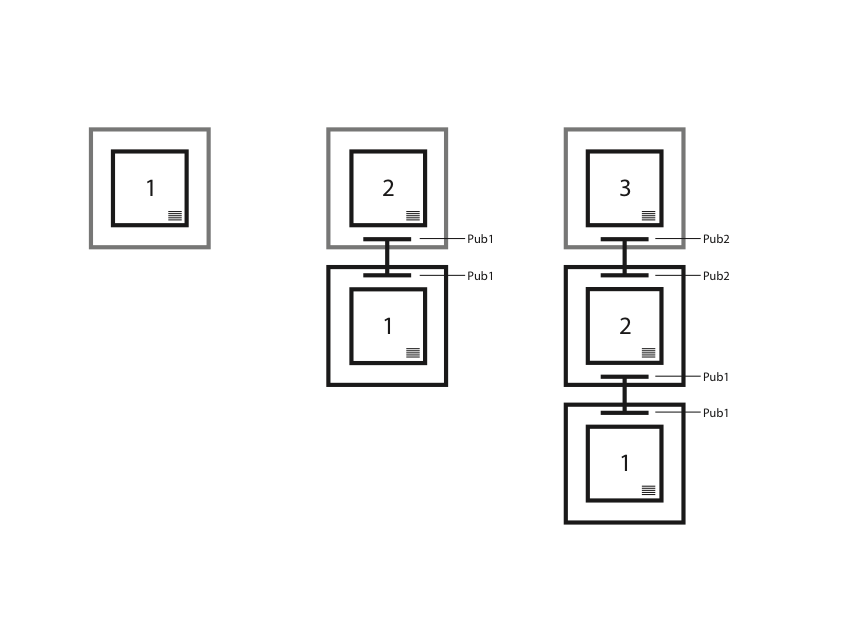
\includegraphics[width=\textwidth] {proofoforigin}
\begin{center}\textbf{Figure 3.}  Link inclusion example in a Proof of Origin Chain
\end{center}

\subsection {Summary}
Given a series of data packets that are signed in sequential pairs with temporary private keys and include the paired public keys, it can be determined with absolute \gls{certainty} that the packets came from the same origin.
%********
%End Proof of Origin
%********
\begin{center}
\line(1,0){50}
\end{center}



%Use Cases Section
\addcontentsline{toc}{section}{Use Cases}
\section*{Use Cases}
From straightforward to complex, the \Gls{xyo-network}'s usage  has vast applications that span a multitude of industries. Take for example an eCommerce Company that could offer its premium customers payment-upon-delivery services. To be able to offer this service, the eCommerce company would leverage the XYO Network and XY Platform (which uses XYO Tokens) to write a \gls{smart-contract} (i.e. on Ethereum's platform). The XYO Network could then track the location of the package being sent to the consumer along every single step of fulfillment; from the warehouse shelf to the the shipping courier, all the way into the consumer's house and every location in between. This could enable eCommerce retailers and websites to verify, in a trustless way, that the package not only appeared on the customer's doorstep, but also safely inside their home. Once the package has arrived in the customer's home (defined and verified by a specific XY-Coordinate), the shipment is considered complete and the payment to the vendor gets released. The eCommerce integration of the XYO Oracle Network thusly enables the ability to protect the merchant from fraud and ensure consumers only pay for goods that arrive in their home.

Consider an entirely different integration of the XYO Network with a hotel review site, whose current problem is that their reviews are often not trusted. Naturally, hotel owners are incentivized to improve their reviews at any cost. What if one could say with extremely high \gls{certainty} that someone was in San Diego, flew to a hotel in Bali and stayed there for two weeks, returned to San Diego, and then wrote a review about their hotel stay in Bali? The review would have a very high reputation, especially if it was written by a serial reviewer who has written many reviews with verified location data. The solutions the XYO Network can provide are infinite and the potential is unlimited.
\begin{center}
\line(1,0){50}
\end{center}




\begin{center}
\line(1,0){50}
\end{center}

\section {Origin Chains}
\Glspl{origin-chain} are the key to verifying that ledgers flowing into the \Gls{xyo-network} are valid. A unique ID for source of data is not practical since it can be forged. Private Key signing is not practical since most parts of the XYO Network are difficult or impossible to physically secure, thus the ability for a bad actor to steal a Private Key is too feasible. To solve this, XYO Network uses \Glspl{transient-key-chain}. The benefit of this is that it is impossible to falsify the chain of origin for data. However, once the chain is broken, it is broken forever and cannot be continued, rendering it an island. 

Every time a \gls{heuristic} ledger is handed off in XYO Network, the receiver appends their own \Gls{proof-of-origin}, which makes the Proof of Origin Ball bigger and generates a Proof of Origin Intersection. Proof of Origin Chains and Proof of Origin Intersections are the primary indicators used by \Glspl{diviner} to verify validity of ledgers. The equation for a Ledger Reputation is effectively what percent of the XYO Network was involved in making the Proof of Origin Ball associated with it. In theory, if 100 percent of the XYO Network records are linked with Proof of Origin and then fully analyzed, the odds of it being valid is 100 percent. If 0 percent of XYO Network records are available for analysis, then validity drops to 0 percent.

For added security, the Public Key for a Chain Link is not provided until the second entry for it is made available. This allows for the time interval between entries or other data to be added to the link.

\subsection {Origin Chain Score}
\Gls{origin-chain-score} is calculated as follows (default algorithm):

\begin{itemize}
\item PcL = \Gls{proof-of-origin} Chain Length
\item PcD = Proof of \Gls{origin-chain} Difficulty
\item Pc' Pc'' O = Proof of Origin Chain Overlap for Pc' and Pc''
\end{itemize}

\begin{equation*}\tag{1} \label{eq1}
Score = \prod_{i=0}^{i=n} \frac{PcL*PcD}{Pc' Pc'' O}
\end{equation*}

\subsection {Origin Tree}
An \Gls{origin-tree} is used to calculate the approximate validity of an answer. It uses the data gathered to generate an Ideal Tree, which is the tree that best fits that data for a given asserted answer. If Node N is located at X,Y,Z,T location, the error across all the data in the set must hold a certain value. To compute this error, we would calculate the MIN, MAX, MEAN, MEDIAN, and AVERAGE DISTANCE FROM THE MEAN.

The asserted answer that has the highest: [Difficulty * (1 - percent error)], is the Best Answer. Using the Proof of Origin Tree, we can identify and prune impossible branches.

\subsection {Reward for Diversity}
The \Gls{xyo-network}'s natural defense against team play is that it holds higher regard for a ledger with a more diverse \Gls{proof-of-origin}. For example, multiple \glspl{heuristic} that have Proof of Origin from the same sources are penalized while multiple heuristics that have diverse Proof of Origin are rewarded. This forces an attacker to have a number of devices so large that is is not economically viable.

\subsection {Privacy}
\Gls{xyo-network} stores all the Ledger Chains as public data in the \Glspl{archivist}. This creates the possibility of inferred data that is associated with people or things to be used nefariously.

\begin{center}
\line(1,0){50}
\end{center}

\section {XYO Network Economy}
\begin{abstract}
The development of decentralized trustless applications has been gaining substantial momentum in recent years, and has now been established as an area for development and research in the field of Computer Science. \Glspl{oracle} are a significant portion of the power and infrastructure needs for decentralized applications, with most of the focus revolving around the connectivity and aggregation of authoritative oracles. We believe that the need for a full featured, fully decentralized and trustless system of oracles is needed for decentralized applications to reach their maximum potential.
\end{abstract}

\subsection {XYO Token: Cryptoeconomics}
The most fascinating notion at the center of cryptocurrency rests the concept of ``\gls{cryptoeconomics}.'' By implementing a Token or currency in one's platform, one can use cryptography to definitively prove past transactions. Then, through game theory and economics incorporated into the design of blockchain protocols, the system incentivizes actors to take the desired human behavior. Similar to how the Ethereum Platform's currency, Ether (ETH), is used as utility to compute and execute transactions, called ``\gls{gas},'' the \Gls{xyo-network} has its own currency, called the XYO Token (XYO). Using XYO, the XYO Network leverages cryptoeconomics to incentivize the desired behavior of providing accurate, reliable location \glspl{heuristic}. XYO Tokens can be thought of as``gas'' needed for one's smart contract to call out and travel through the real world in order to verify the XY-coordinate of a specified object.

The process works like this: A token holder queries the XYO Network by asking a question, (e.g.``Where is my Amazon package with XYO Address 0xe0EbD...e34a''). The question gets sent into a queue, where it waits to be processed and answered. Similar to how in Ethereum, one sets their Gas Limit and Gas Price, one can set their own XYO Gas Limit and XYO Gas Price. The higher one sets their XYO Gas Limit and XYO Gas Price, the higher priority their question will have in the queue. The XY Component that answers the query is the \Gls{diviner}. The cost of a question (in XYO tokens) is determined by the amount of data required to provide an answer to the query.  The more data needed, the more expensive the question and higher the XYO Gas Price. Potential queries to the XYO Network are infinite. For instance, a trucking and logistics company could query the XYO Network to ask, ``What is the location of every single car in our fleet?''

Once the XYO Token holder queries the XYO Network and pays the requested gas, the Diviner calls out to the relevant \Gls{archivist} to retrieve the pertinent data needed to answer the query. The data returned is derived from the \Glspl{bridge}, who originally gathered the data from the \Glspl{sentinel}. Sentinels are essentially devices or signals that verify the location of objects. These include devices like Bluetooth trackers, GPS trackers, geo-location tracking built into IoT devices, satellite tracking technology, QR-code scanners, RFID scanning and many others. XY Findables has pioneered and launched its consumer business, XY Find It, which has allowed it to test and process real-world location heuristics. All efforts of XY Find It have served to help significantly in designing the XYO Network Blockchain Protocol.

If the data provided by a Sentinel device (i.e. XY Find It Beacon) is used to answer a query, then all four Components involved in the transaction receive a part of the XYO Gas paid by the token holder: the Diviner (who searched for the answer), the Archiver (who stored the data), the Bridge (who transmitted the data) and the Sentinel (who recorded the location data)receive a part of the XYO Gas paid by the token holder. The distribution of the gas between the 4 components of the XYO Network always happens in the same proportion.  Within each component, gas gets distributed evenly.

% TODO: 
\subsection {Cryptoeconomics: Intent-testing and Ideal-state Intelligence}

\subsection {Beyond XY Find It Bluetooth \& GPS Tracking Sentinels}
The \Gls{xyo-network} is engaging with businesses to expand its network of \Glspl{sentinel} beyond its own network of XY Find It beacons, which total to over 800,000 globally as of January 2018. A variety of devices can act as Sentinels. Generally, the greater the Sentinel cardinality in the XYO Network, the more reliable the network. To broaden and strengthen the XYO Network, we are currently engaging mobile app companies, IoT companies and hardware companies to add Sentinels to the XYO Network. The XYO Network is providing solutions to a plethora of industries including eCommerce, government, automotive, healthcare, pharmaceutical, construction, insurance, utilities, oil \& gas, supply chain \& logistics, as well as businesses specializing in goods \& services reviews and traditional brick \& mortar retail. XY is working with a vast array of companies in order to create strategic partnerships that leverage \gls{cryptoeconomics} and economic incentives that are beneficial to both the Partner and end-user (which ultimately provide a cheaper product or service for the consumer).

\subsection {XYO Token Specifications}
\begin{itemize}
\item Smart contract platform: Ethereum
\item Contract Type: ERC-20
\item Token: XYO
\item Token Name: \Gls{xyo-network} Utility Token
\item Token Address: 0x55296f69f40ea6d20e478533c15a6b08b654e758
\item Total issuance: Finite and capped at the amount reached after the Token Main Sale
\item Amount issued during the main sale: Unlimited
\item Unsold and Unallocated tokens: Burned after the token sale event. No further XYO tokens will be generated after the Main Sale ends.
\end{itemize}

\begin{center}
\line(1,0){50}
\end{center}

\section {Bound Witness}
\begin{abstract}
Given that an untrusted source of data for the use of digital contract resolution (an \gls{oracle}) is not useful, we can substantially increase the \gls{certainty} of the data provided by first establishing the existence of a bidirectional \gls{heuristic}. The primary bidirectional heuristic is proximity since both parties can validate the occurrence and range of an interaction by cosigning the interaction. This allows for a zero-knowledge proof that the two nodes were in proximity of each other.
\end{abstract}

\subsection {Goal}
Determine the \gls{certainty} that an \gls{oracle} witness node in a trustless system gathered the data that it is sharing.

\subsection {Problem}
In a trustless system, a witness node can either by defect or corruption produce false data. Invalid data can be detected and removed simply if it falls outside the allowed range for that \gls{heuristic}. Valid but incorrect data (i.e. false data) is much more difficult to detect. 

\subsection {Unidirectional vs. Bidirectional Heuristics}
Most \glspl{heuristic} are unidirectional. This means that the element being measured cannot measure back, making heuristic data very difficult to validate. A bidirectional heuristic is one where the measured element measures back and reports on the other party which makes validation possible. Location is a rare heuristic in that it can be bidirectional with two edge nodes reporting on each other. A real-world example of this would be if two people who are near each other take a selfie, print a copy for each party, and then both sign the selfie, giving both parties Proof of Proximity. The only way for the two to have gotten this ``data'' would be for them to have been together.

\subsection {Network Effect}
Imagine a system where every edge node is expected to constantly produce these ``selfies'' as they travel around, and store them in a binder. They are also expected to keep that binder in time-sequential order and are never allowed to delete one. This establishes a proximity recorder for each edge node that can be cross referenced with the recorders of the other edge nodes.

\subsection {Non-Edge Nodes}
All nodes are considered ``witnesses'', including bridge, relay, storage, and analysis nodes. This allows for any data that is relayed from one node to the next to be bound. This is the concept of the \Gls{bound-witness}.

\subsection {Cross Reference}
Analyzing every set of ``selfies'' that is produced and chained together by every edge node allows the system to produce the Best Answer from the relative proximity of all the nodes that are in the network. If every node reports honestly and accurately, the mapping of all the relative positions of the edge nodes will achieve the maximum \gls{certainty} and \gls{accuracy} possible: 100 percent. Conversely, if every node either is dishonest or flawed, the certainty and accuracy both can approach the minimum of 0 percent.

Given a set of reported data and a query for a relative position of one of the edge nodes, an approximation of the position and a certainty and accuracy coefficient can be generated.

Given the same set of data and the same analysis algorithm, every calculation should arrive at the same position approximation and certainty and accuracy coefficients.

\subsection {Diagram}
S' and S'' (Figure 2.) are each a \Gls{sentinel} (edge node) that collect \glspl{heuristic}. When in contact with each other, they exchange heuristic data and public keys. Both build a full record of the interaction and sign the resulting interaction. That signed record then becomes the next entry in both of their local ledgers (16 for S' and 3 for S''). This action binds these two witnesses as being within proximity of each other.

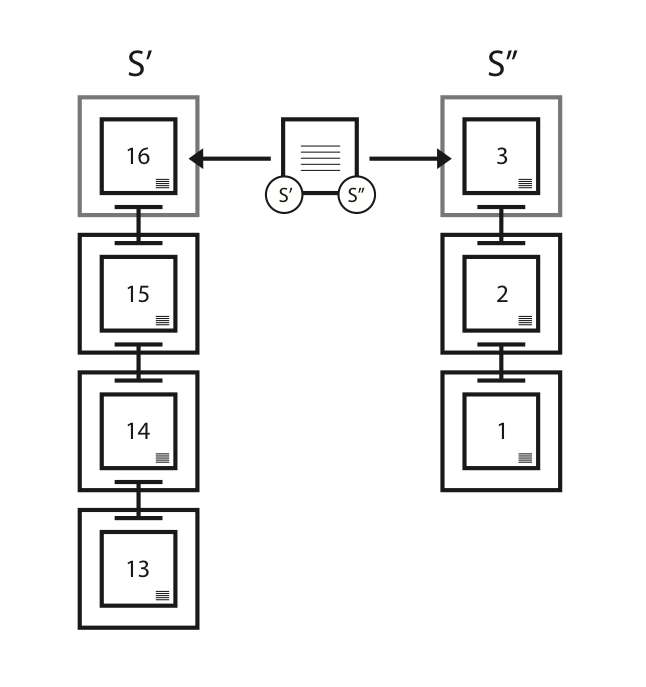
\includegraphics [width=\textwidth]{boundwitness}
\begin{center}\textbf{Figure 2.}  Record logging example between two Sentinels
\end{center}

\subsection {Summary}
Given a network of edge nodes that can collect signed, time-sequenced, bidirectional \glspl{heuristic}, a relative proximity between any two edge nodes can be established with a high level of confidence and \gls{accuracy}.

\begin{center}
\line(1,0){50}
\end{center}



\clearpage


%*******************************
%**** Begin Glossary Section *****
%*******************************

\newglossaryentry{sentinel}
{
    name={Sentinel},
    description={A Sentinel is a heuristic witnesses. It observes heuristics and vouches for the certainty and accuracy of them by producing temporal ledgers. The most important aspect of a Sentinel is that it produces ledgers that Diviners can be certain came from the same source by adding Proof of Origin to them}
}

\newglossaryentry{bridge}
{
    name={Bridge},
    description={A Bridge is a heuristic transcriber. It securely relays heuristic ledgers from Sentinels to Diviners. The most important aspect of a Bridge is that a Diviner can be sure that the heuristic ledgers that are received from a Bridge have not been altered in any way. The second most important aspect of a Bridge is that they add an additional Proof of Origin metadata}
}

\newglossaryentry{archivist}
{
    name={Archivist},
    description={An Archivist stores heuristics as a part of the decentralized data set with the goal of having all historical ledgers stored, but without that requirement. Even if some data is lost or becomes temporarily unavailable, the system continues to function, just with reduced accuracy. Archivists also index ledgers so that they can return a string of ledger data if needed. Archivists store raw data only and get paid solely for retrieval of the data. Storage is always free}
}

\newglossaryentry{diviner}
{
    name={Diviner},
    description={A Diviner answers a given question by analyzing historical data that has been stored by the XYO Network. Heuristics stored in the XYO Network must have a high level of Proof of Origin to determine the validity and accuracy of the heuristic. A Diviner obtains and delivers an answer by judging the witness based on its Proof of Origin. Given that the XYO Network is a trustless system, Diviners must be incentivized to provide honest analyses of heuristics. Unlike Sentinels and Bridges, Diviners use Proof of Work to add answers to the blockchain}
}

\newglossaryentry{webble}
{
    name={webble},
    description={Everything in the world is defined spatially by its \textit{X,Y,Z,T} coordinate and nothing can leave that space. Objects are thus confined to ``webbubbles'', or what are referred to as \textit{webbles}.}
}

\newglossaryentry{gas}
{
    name={gas},
    description={The cost of a transaction (i.e. question) in the form of XYO Tokens}
}

\newglossaryentry{proof-of-origin}
{
    name={Proof of Origin},
    description={Proof of Origin is the key to verifying that ledgers flowing into the XYO Network are valid. A unique ID for source of data is not practical since it can be forged. Private Key signing is not practical since most parts of the XYO Network are difficult or impossible to physically secure, thus the potential for a bad actor to steal a Private Key is too feasible. To solve this, XYO Network uses Transient Key Chaining. The benefit of this is that it is impossible to falsify the chain of origin for data. However, once the chain is broken, it is broken forever and cannot be continued, rendering it an island}
}

\newglossaryentry{proof-of-work}
{
    name={Proof of Work},
    description={Proof of Work is a piece of data that satisfies certain requirements, is difficult to produce (i.e. costly, time-consuming), but easy for others to verify. Producing a Proof of Work can be a random process with a low probability of generation so that rigorous trial and error is required on average before a valid Proof of Work is created}
}

\newglossaryentry{bound-witness}
{
    name={Bound Witness},
    description={Bound Witness is a concept achieved by the existence of a bidirectional heuristic. Given that an untrusted source of data for the use of digital contract resolution (an oracle) is not useful, there is a substantial increase in certainty of the data provided by the establishment of such a heuristic. The primary bidirectional heuristic is proximity since both parties can validate the occurrence and range of an interaction by cosigning the interaction. This allows for a zero-knowledge proof that the two nodes were in proximity of each other.}
}

\newglossaryentry{smart-contract}
{
    name={smart contract},
    description={A protocol coined by Nick Szabo before Bitcoin, purportedly in 1994 (which is why some believe him to be Satoshi Nakamoto, the mystical and unknown inventor of Bitcoin). The idea behind smart contracts is to codify a legal agreement in a program and to have decentralized computers execute its terms, instead of humans having to interpret and act on contracts. Smart contracts collapse money (e.g. Ether) and contracts into the same concept. Being that smart contracts are deterministic (like computer programs) and fully transparent and readable, they serve as a powerful way to replace middle-men and brokers}
}

\newglossaryentry{cryptoeconomics}
{
    name={cryptoeconomics},
    description={A formal discipline that studies protocols that govern the production, distribution, and consumption of goods and services in a decentralized digital economy. Cryptoeconomics is a practical science that focuses on the design and characterization of these protocols}
}

\newglossaryentry{xyo-network}
{
    name={XYO Network},
    description={XYO Network stands for "XY Oracle Network." It is comprised of the entire system of XYO enabled components/nodes that include Sentinels, Bridges, Archivists, and Diviners. The primary function of the XYO Network is to act as a portal by which digital smart contracts can be executed through real world geo-location confirmations}
}

\newglossaryentry{certainty}
{
    name={certainty},
    description={A measure of the likelihood that a data point or heuristic is free from corruption or tampering}
}

\newglossaryentry{accuracy}
{
    name={accuracy},
    description={A measure of confidence that a data point or heuristic is within a specific margin of error}
}

\newglossaryentry{oracle}
{
    name={oracle},
    description={A part of a DApp (decentralized application) system that is responsible for resolving a digital contract by providing an answer with accuracy and certainty. The term ``oracle'' originates from cryptography where it signifies a truly random source (e.g. of a random number). This provides the necessary gate from a crypto equation to the world beyond. Oracles feed smart contracts information from beyond the chain (the real world, or off-chain). Oracles are interfaces from the digital world to the real world. As a morbid example, consider a contract for a Last Will \& Testament. A Will's terms are executed upon confirmation that the testator is deceased. An oracle service could be built to trigger a Will by compiling and aggregating relevant data from official sources. The oracle could then be used as a feed or end-point for a smart contract to call out to in order to check whether or not the person is deceased}
}

\newglossaryentry{heuristic}
{
    name={heuristic},
    description={A data point about the real world relative to the position of a Sentinel (proximity, temperature, light, motion, etc...)}
}

\newglossaryentry{transient-key-chain}
{
    name={Transient Key Chain},
    description={A Transient Key Chain links a series of data packets using Transient Key Cryptography}
}

\newglossaryentry{best-answer-score}
{
    name={Best Answer Score},
    description={A score generated by a Best Answer Algorithm that ranks the quality of the score.  The higher the score, the better it is, per the algorithm.  This score is used to determine which answer is better given two analyzed answers}
}

\newglossaryentry{best-answer-algorithm}
{
    name={Best Answer Algorithm},
    description={An algorithm used to generate Best Answer Scores when a Diviner chooses an answer.  The XYO Network permits the addition of specialized algorithms and allows the customer to specify which algorithm to use.  It is required that this algorithm will result in the same score when run on any Diviner given the same data set}
}

\newglossaryentry{origin-chain-score}
{
    name={Origin Chain Score},
    description={The score assigned to an Origin Chain to determine its credibility. This assessment takes length, tangle, overlap, and redundancy into consideration}
}

\newglossaryentry{origin-chain}
{
    name={Origin Chain},
    description={A Transient Key Chain that links together a series of Bound Witness heuristic ledger entries}
}

\newglossaryentry{origin-tree}
{
    name={Origin Tree},
    description={A data set of ledger entries taken from various Origin Chains to establish the origin of a heuristic ledger entry with a specified level of certainty}
}

\newacronym{pow}{PoW}{Proof of Work}

\newacronym{poo}{PoO}{Proof of Origin}

\newacronym{xy-oracle-network}{XY Oracle Network}{XYO Network}

\printglossaries

%*******************************
%**** End Glossary Section *****
%*******************************




\end{document}
